\documentclass[12pt]{article}
\usepackage[letterpaper, portrait, margin=1in]{geometry}
\PassOptionsToPackage{hyphens}{url}\usepackage{hyperref}
\usepackage{graphicx}
\usepackage[colorinlistoftodos]{todonotes}
\usepackage{xcolor}
\usepackage{soul}

\graphicspath{{images/}}

\newcommand{\alert}[1]{\todo[color=red!40]{#1}}
\newcommand{\edit}[1]{\todo[color=yellow!60]{#1}}
\newcommand{\question}[1]{\todo[color=cyan!40]{#1}}

\begin{document}
\sloppy

\include{transmittalletter}

% \begin{titlepage}
    \begin{center}
        \vspace*{1cm}

    \end{center}
\end{titlepage}
% \begin{titlepage}
    \begin{center}
        \vspace*{1cm}

        \LARGE
        \textbf{CPU-Sim}

        \vspace{0.5cm}
        \Large
        Code Documentation
        
        \vspace{2cm}

        \textbf{Author: Benjamin Talbot}
        
        \vspace{0.5cm}
        June 23, 2024

        % \normalsize
        % \vspace{5cm}
        % text\\
        % \vspace{0.25cm}
        % text

        % \vspace{5.5cm}
        % text\\
        % text\\
        % text\\
    \end{center}
\end{titlepage}

\newpage

\section{Introduction}


\section{Components}


\section{Graphics}

\begin{figure}
    \centering
    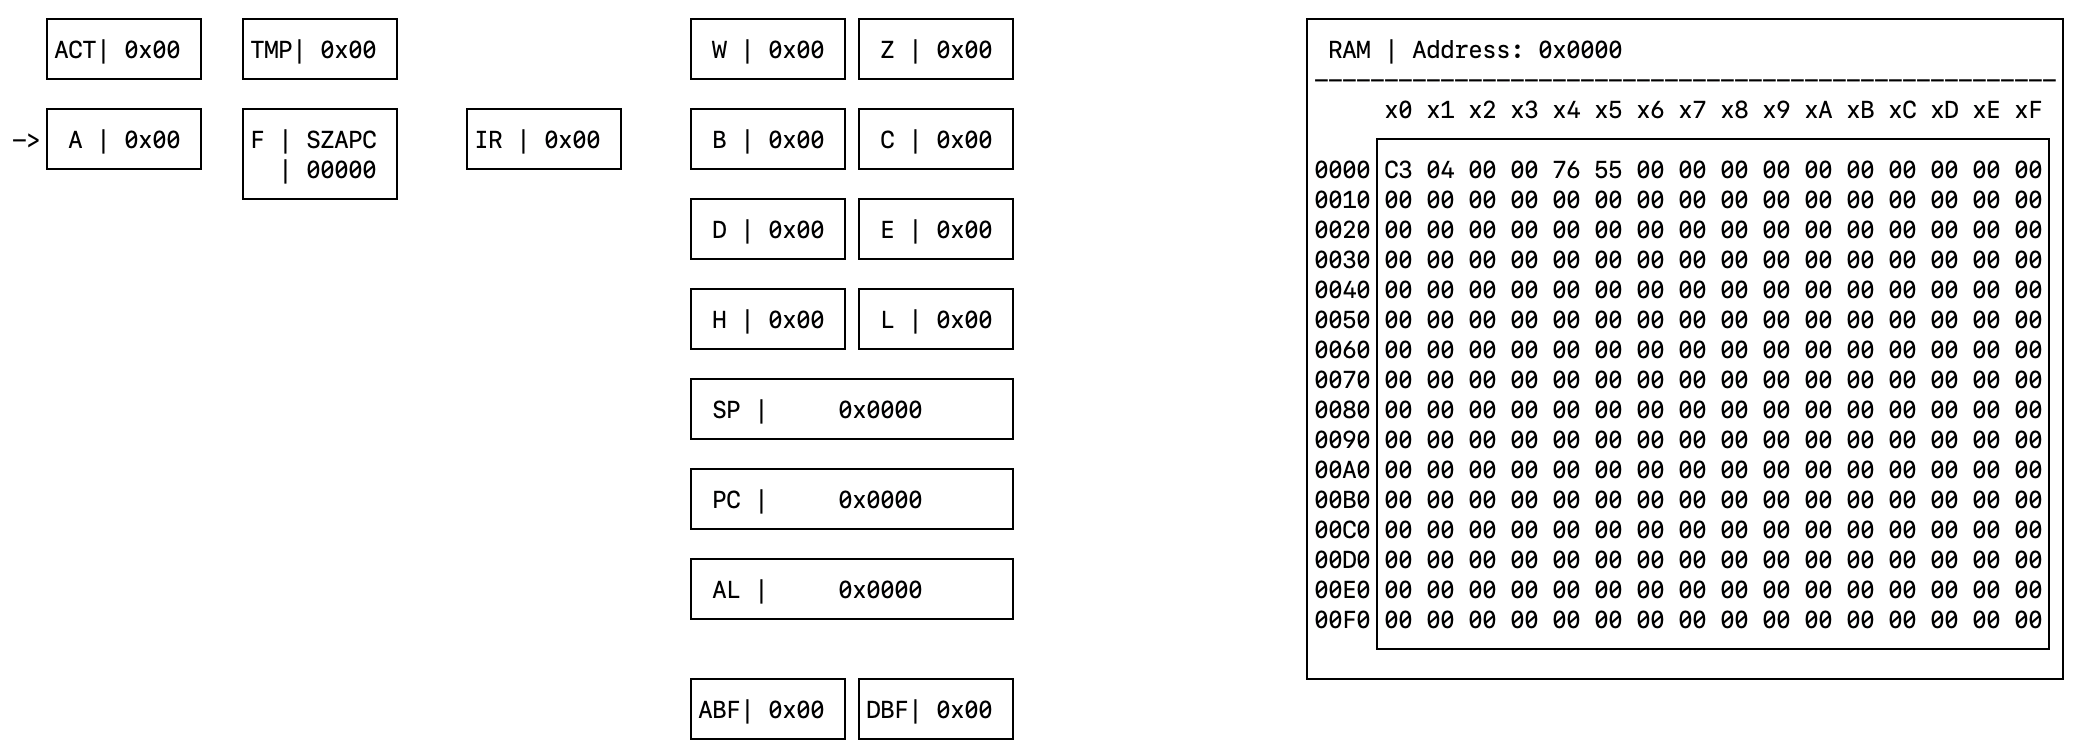
\includegraphics[scale=0.45]{layout.png}
    \caption{Layout of the system}
    \label{fig:layout}
\end{figure}
\section{Graphics}

\begin{figure}
    \centering
    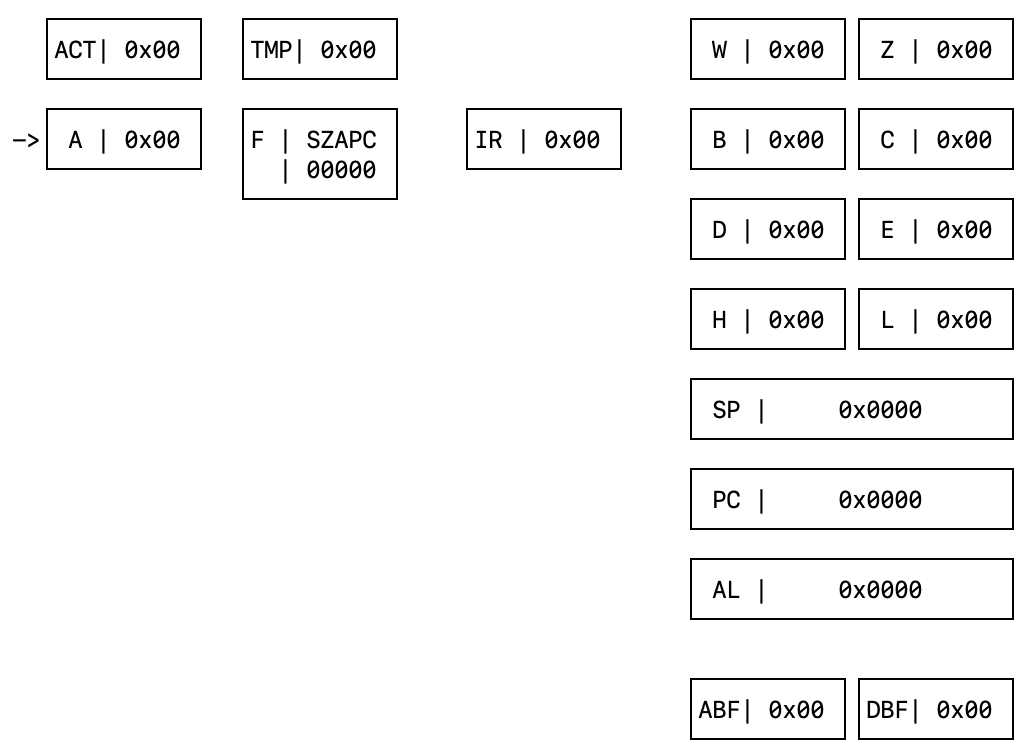
\includegraphics[scale=0.9]{intel8080.png}
    \caption{Intel 8080}
    \label{fig:intel8080}
\end{figure}
\section{Graphics}

\begin{figure}
    \centering
    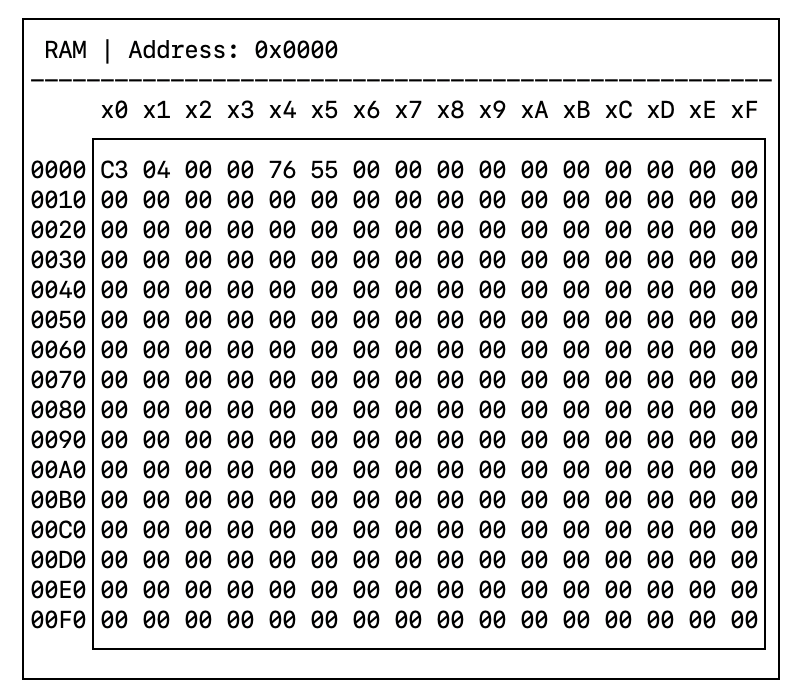
\includegraphics[scale=1]{ram.png}
    \caption{RAM}
    \label{fig:ram}
\end{figure}

% 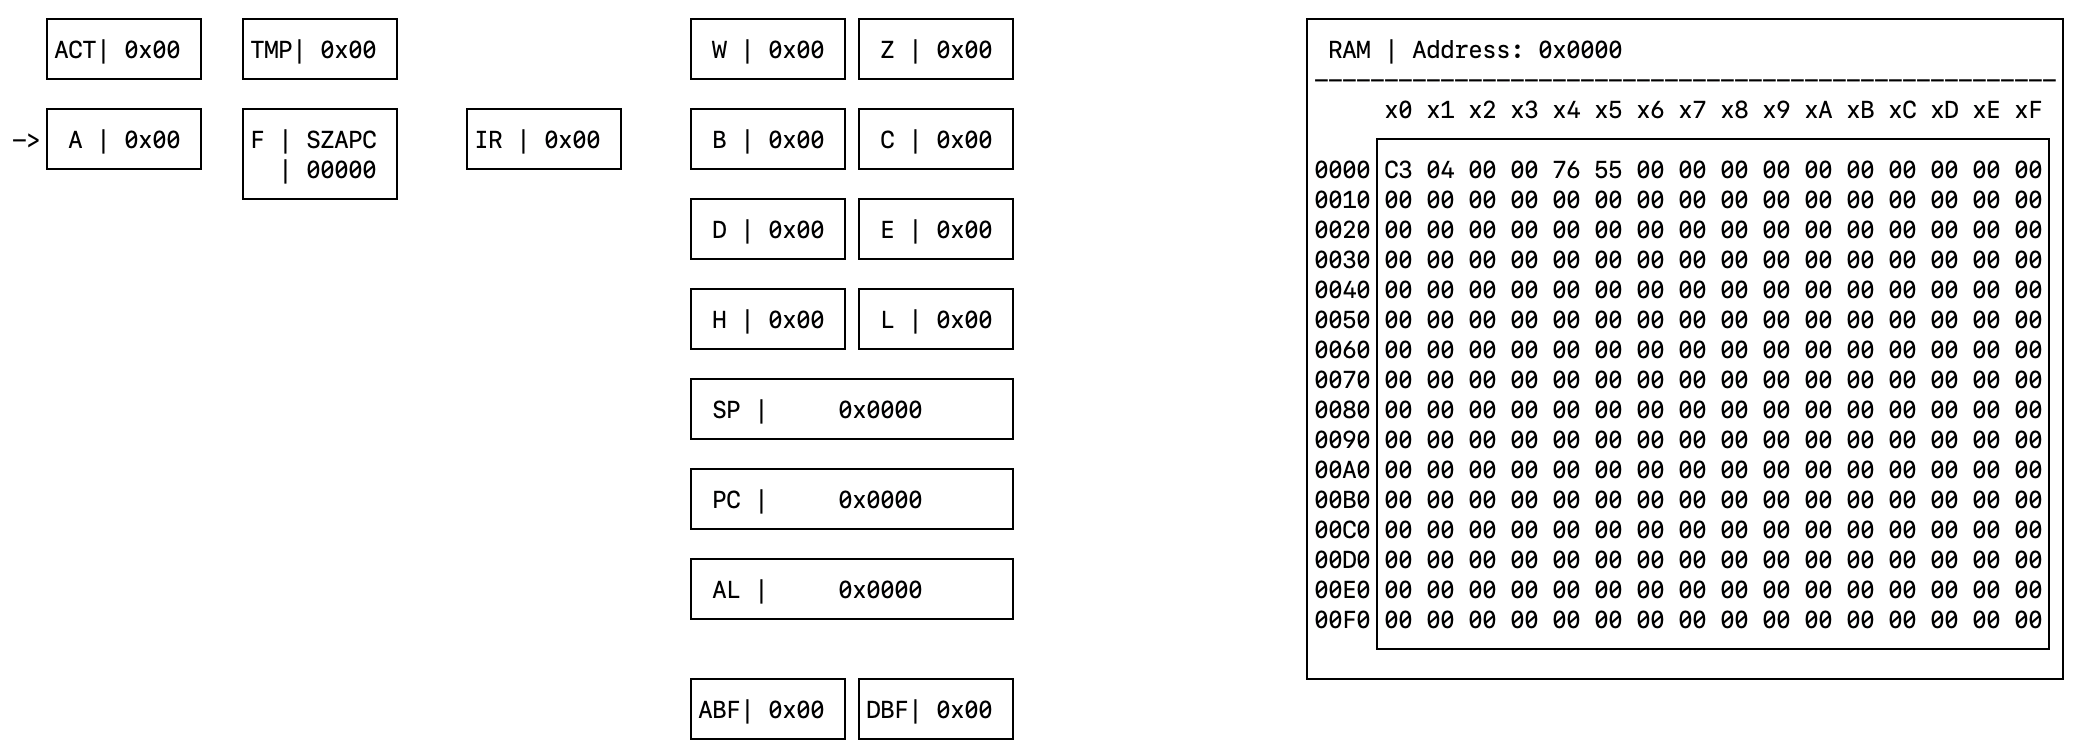
\includegraphics{layout.png}




\end{document}
